\documentclass{article}
\usepackage{amsmath}
\usepackage{amsthm}
\usepackage{amssymb}
\usepackage{subcaption}
\usepackage{tikz}
\usepackage{float}

\title{Production Technologies (supplementary)}

\begin{document}
%\maketitle

\begin{enumerate}
    \item[3.] No free lunch: $Y \cap \mathbb{R}^L_{+} \subseteq \{0\}$
    \begin{figure}[h]
        \centering
        \begin{subfigure}{.5\textwidth}
            \centering
            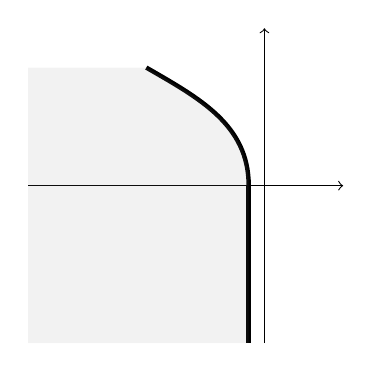
\begin{tikzpicture}[fill opacity=0.1,draw opacity=1]
                \draw [->] (-3,0) -- (1,0);
                \draw [->] (0,-2) -- (0,2);
                \draw [ultra thick] (-0.2,0) -- (-0.2,-2);
                \draw [ultra thick] (-1.5,1.5) to [out=-30,in=90](-0.2,0);
                \path [fill=gray,fill opacity=.1] (-3,1.5) -- (-1.5,1.5) to [out=-30,in=90] (-0.2,0) -- (-0.2,-2) -- (-3,-2) -- (-3,1.5);
            \end{tikzpicture}
            \caption{no free lunch}
        \end{subfigure}%
        \begin{subfigure}{.5\textwidth}
            \centering
            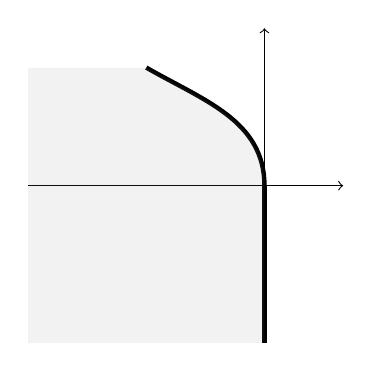
\begin{tikzpicture}
                \draw [->] (-3,0) -- (1,0);
                \draw [->] (0,-2) -- (0,2);
                \draw [ultra thick] (0,0) -- (0,-2);
                \draw [ultra thick] (-1.5,1.5) to [out=-30,in=90](0,0);
                \path [fill=gray,fill opacity=.1] (-3,1.5) -- (-1.5,1.5) to [out=-30,in=90] (0,0) -- (0,-2) -- (-3,-2) -- (-3,1.5);
            \end{tikzpicture}
            \caption{violation of no free lunch}
        \end{subfigure}
    \end{figure}
    
    \item[5.] Free disposal: $y'\leq y \in Y \implies y' \in Y$
    \begin{figure}[h]
        \centering
        \begin{subfigure}{.5\textwidth}
            \centering
            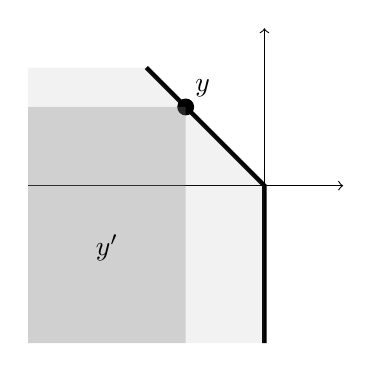
\begin{tikzpicture}
                \draw [->] (-3,0) -- (1,0);
                \draw [->] (0,-2) -- (0,2);
                \draw [ultra thick] (-1.5,1.5)--(0,0)--(0,-2);
                \path [fill=gray,fill opacity=.1] (-3,1.5)--(-1.5,1.5)--(0,0)--(0,-2)--(-3,-2)--(-3,-1.5);
                \draw [fill] (-1,1) circle [radius=0.1];
                \path [fill=gray, fill opacity=.3] (-3,1)--(-1,1)--(-1,-2)--(-3,-2)--(-3,1);
                \node [above right] at (-1,1) {$y$};
                \node [below] at (-2,-0.5) {$y'$};
            \end{tikzpicture}
            \caption{free disposal}
        \end{subfigure}%
        \begin{subfigure}{.5\textwidth}
            \centering
            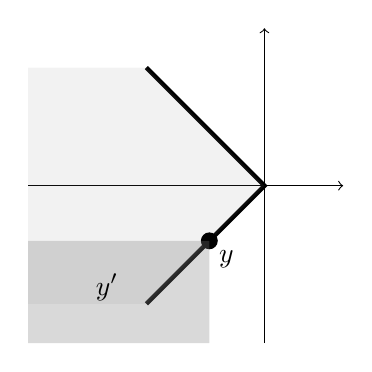
\begin{tikzpicture}
                \draw [->] (-3,0) -- (1,0);
                \draw [->] (0,-2) -- (0,2);
                \draw [ultra thick] (-1.5,1.5)--(0,0)--(-1.5,-1.5);
                \path [fill=gray,fill opacity=.1] (-3,1.5)--(-1.5,1.5)--(0,0)--(-1.5,-1.5)--(-3,-1.5)--(-3,1.5);
                \draw [fill] (-0.7,-0.7) circle [radius=.1];
                \path [fill=gray, fill opacity=.3] (-3,-0.7)--(-0.7,-0.7)--(-0.7,-2)--(-3,-2)--(-3,-0.7);
                \node [below right] at (-0.7,-0.7) {$y$};
                \node [below] at (-2, -1) {$y'$};
            \end{tikzpicture}
            \caption{violation of free  disposal}
        \end{subfigure}
    \end{figure}
    
    \item[6.] Irreversible: $y \in Y \implies -y\not\in Y$
    \begin{figure}[H]
        \centering
        \begin{subfigure}{.5\textwidth}
            \centering
            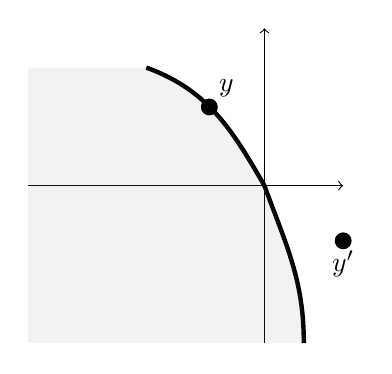
\begin{tikzpicture}
                \draw [->] (-3,0) -- (1,0);
                \draw [->] (0,-2) -- (0,2);
                \draw [ultra thick] (-1.5,1.5) to [out=-20,in=120] (0,0);
                \draw [ultra thick] (0,0) to [out=-70,in=90] (0.5,-2);
                \path [fill=gray,fill opacity=.1] (-3,1.5)--(-1.5,1.5) to [out=-20,in=120] (0,0) to [out=-70,in=90] (0.5,-2)--(-3,-2)--(-3,1.5);
                \draw [fill] (-0.7,1) circle [radius=.1];
                \draw [fill] (1,-0.7) circle [radius=.1];
                \node [above right] at (-0.7,1) {$y$};
                \node [below] at (1,-0.7) {$y'$};
            \end{tikzpicture}
            \caption{irreversible}
        \end{subfigure}%
        \begin{subfigure}{.5\textwidth}
            \centering
            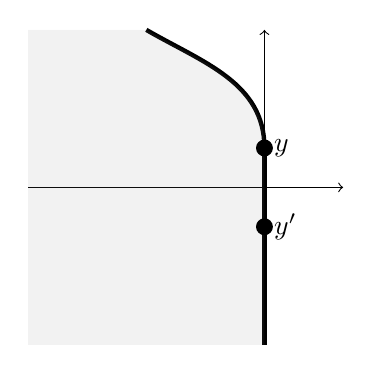
\begin{tikzpicture}
                \draw [->] (-3,0) -- (1,0);
                \draw [->] (0,-2) -- (0,2);
                \draw [ultra thick] (0,0.5) -- (0,-2);
                \draw [ultra thick] (-1.5,2) to [out=-30,in=90](0,0.5);
                \path [fill=gray,fill opacity=.1] (-3,2) -- (-1.5,2) to [out=-30,in=90] (0,0.5) -- (0,-2) -- (-3,-2) -- (-3,1.5);
                \draw [fill] (0,0.5) circle [radius=0.1];
                \draw [fill] (0,-0.5) circle [radius=0.1];
                \node [right] at (0,0.5) {$y$};
                \node [right] at (0,-0.5) {$y'$};
            \end{tikzpicture}
            \caption{violation of irreversible}
        \end{subfigure}
    \end{figure}
    
    \newpage
    \item[7.] Non-increasing returns to scale: $y \in Y \implies  ay \in Y\ \forall a \in [0,1]$
    \begin{figure}[H]
        \centering
        \begin{subfigure}{.5\textwidth}
            \centering
            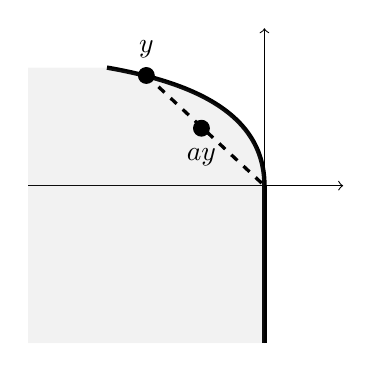
\begin{tikzpicture}
                \draw [->] (-3,0) -- (1,0);
                \draw [->] (0,-2) -- (0,2);
                \draw [ultra thick] (-2,1.5) to [out=-10,in=90] (0,0);
                \draw [ultra thick] (0,0)--(0,-2);
                \path [fill=gray,fill opacity=.1] (-3,1.5)--(-2,1.5) to [out=-10,in=90] (0,0)--(0,-2)--(-3,-2)--(-3,1.5);
                \draw [fill] (-1.5,1.4) circle [radius=.1];
                \draw [very thick, dashed] (-1.5,1.4)--(0,0);
                \draw [fill] (-0.8,0.73) circle [radius=.1];
                \node [above] at (-1.5,1.5) {$y$};
                \node [below] at (-0.8,0.6) {$a y$};
            \end{tikzpicture}
            \caption{NIRTS}
        \end{subfigure}%
        \begin{subfigure}{.5\textwidth}
            \centering
            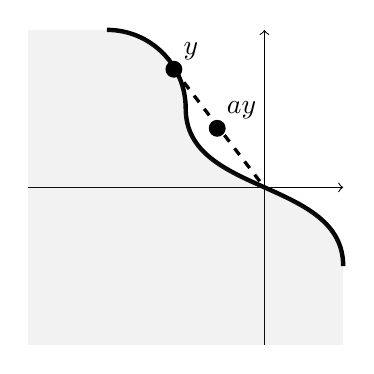
\begin{tikzpicture}
                \draw [->] (-3,0) -- (1,0);
                \draw [->] (0,-2) -- (0,2);
                \draw [ultra thick] (-2,2) to [out=0,in=90] (-1,1) to [out=-90,in=90] (1,-1);
                \path [fill=gray,fill opacity=.1] (-3,2)--(-2,2) to [out=0,in=90] (-1,1) to [out=-90,in=90] (1,-1)--(1,-2)--(-3,-2)--(-3,2);
                \draw [fill] (-1.15, 1.5) circle [radius=.1];
                \draw [very thick, dashed] (-1.15,1.5)--(0,0);
                \draw [fill] (-0.6,0.75) circle [radius=.1];
                \node [above right] at (-1.15,1.5) {$y$};
                \node [above right] at (-0.6,0.75) {$a y$};
            \end{tikzpicture}
            \caption{violation of NIRTS}
        \end{subfigure}
    \end{figure}

    \item[8.] Non-decreasing returns to scale: $y \in Y \implies  ay \in Y\ \forall a \in [1,\infty)$
    \begin{figure}[H]
        \centering
        \begin{subfigure}{.5\textwidth}
            \centering
            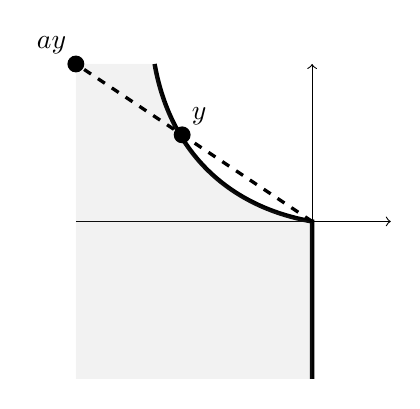
\begin{tikzpicture}
                \draw [->] (-3,0) -- (1,0);
                \draw [->] (0,-2) -- (0,2);
                \draw [ultra thick] (-2,2) to [out=-80, in=170] (0,0)--(0,-2);
                \path [fill=gray,fill opacity=.1] (-3,2)--(-2,2) to [out=-80, in=170] (0,0)--(0,-2)--(-3,-2)--(-3,2);
                \draw [very thick, dashed] (0,0)--(-3,2);
                \draw [fill] (-1.65,1.1) circle [radius=.1];
                \draw [fill] (-3,2) circle [radius=.1];
                \node [above left] at (-3,2) {$a y$};
                \node [above right] at (-1.65,1.1) {$y$};
            \end{tikzpicture}
            \caption{NDRTS}
        \end{subfigure}%
        \begin{subfigure}{.5\textwidth}
            \centering
            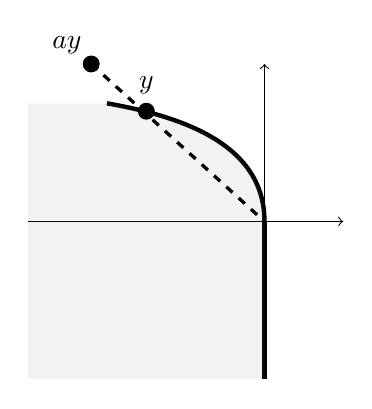
\begin{tikzpicture}
                \draw [->] (-3,0) -- (1,0);
                \draw [->] (0,-2) -- (0,2);
                \draw [ultra thick] (-2,1.5) to [out=-10,in=90] (0,0);
                \draw [ultra thick] (0,0)--(0,-2);
                \path [fill=gray,fill opacity=.1] (-3,1.5)--(-2,1.5) to [out=-10,in=90] (0,0)--(0,-2)--(-3,-2)--(-3,1.5);
                \draw [fill] (-1.5,1.4) circle [radius=.1];
                \draw [very thick, dashed] (-2.2,2)--(0,0);
                \draw [fill] (-2.2,2) circle [radius=.1];
                \node [above] at (-1.5,1.5) {$y$};
                \node [above left] at (-2.2,2) {$a y$};
            \end{tikzpicture}
            \caption{violation of NDRTS}
        \end{subfigure}
    \end{figure}
 
    \item[9.] Constant returns to scale: $y \in Y \implies  ay \in Y\ \forall a \in [0,\infty)$
    \begin{figure}[H]
        \centering
        \begin{subfigure}{.5\textwidth}
            \centering
            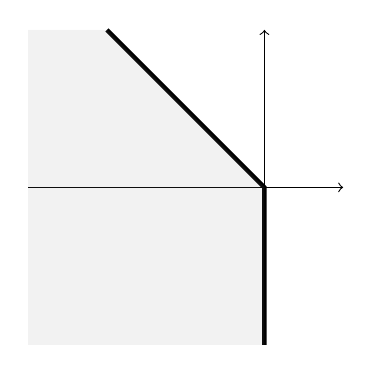
\begin{tikzpicture}
                \draw [->] (-3,0) -- (1,0);
                \draw [->] (0,-2) -- (0,2);
                \draw [ultra thick] (-2,2) --(0,0)--(0,-2);
                \path [fill=gray, fill opacity=.1] (-3,2)--(-2,2) --(0,0)--(0,-2)--(-3,-2)--(-3,2);
            \end{tikzpicture}
            \caption{CRTS}
        \end{subfigure}%
        \begin{subfigure}{.5\textwidth}
            \centering
            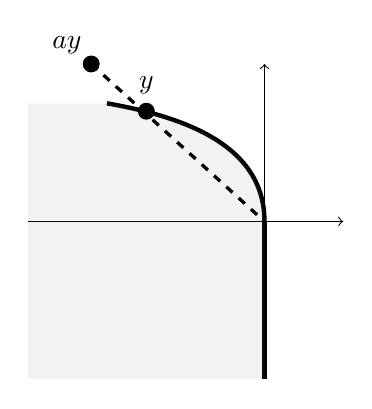
\begin{tikzpicture}
                \draw [->] (-3,0) -- (1,0);
                \draw [->] (0,-2) -- (0,2);
                \draw [ultra thick] (-2,1.5) to [out=-10,in=90] (0,0);
                \draw [ultra thick] (0,0)--(0,-2);
                \path [fill=gray,fill opacity=.1] (-3,1.5)--(-2,1.5) to [out=-10,in=90] (0,0)--(0,-2)--(-3,-2)--(-3,1.5);
                \draw [fill] (-1.5,1.4) circle [radius=.1];
                \draw [very thick, dashed] (-2.2,2)--(0,0);
                \draw [fill] (-2.2,2) circle [radius=.1];
                \node [above] at (-1.5,1.5) {$y$};
                \node [above left] at (-2.2,2) {$a y$};
            \end{tikzpicture}
            \caption{violation of CRTS}
        \end{subfigure}
    \end{figure}
 
    \newpage
    \item[11.] Strict convexity: $y,y' \in Y \implies ay + (1-a)y' \in \textrm{int}(Y)\ \forall a \in (0,1)$
    \begin{figure}[H]
        \centering
        \begin{subfigure}{.5\textwidth}
            \centering
            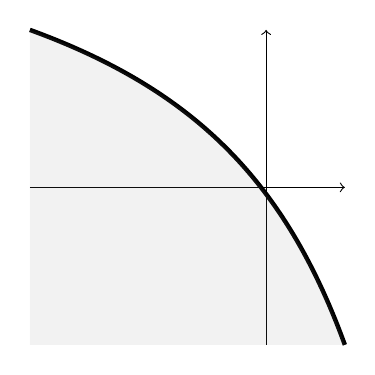
\begin{tikzpicture}
                \draw [->] (-3,0) -- (1,0);
                \draw [->] (0,-2) -- (0,2);
                \draw [ultra thick] (-3,2) to [out=-20, in=110](1,-2);
                \path [fill=gray,fill opacity=.1] (-3,2) to [out=-20,in=110] (1,-2)--(-3,-2)--(-3,2);
            \end{tikzpicture}
            \caption{strictly convexity}
        \end{subfigure}%
        \begin{subfigure}{.5\textwidth}
            \centering
            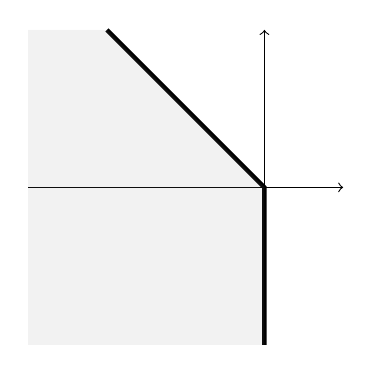
\begin{tikzpicture}
                \draw [->] (-3,0) -- (1,0);
                \draw [->] (0,-2) -- (0,2);
                \draw [ultra thick] (-2,2) --(0,0)--(0,-2);
                \path [fill=gray, fill opacity=.1] (-3,2)--(-2,2) --(0,0)--(0,-2)--(-3,-2)--(-3,2);
            \end{tikzpicture}
            \caption{violation of strictly convexity}
        \end{subfigure}
    \end{figure}      
    
    \item[12.] Convex cone: $y,y' \in Y \implies \alpha y + \beta y' \in Y\ \forall \alpha,\beta \geq 0$
    \begin{figure}[H]
        \centering
        \begin{subfigure}{.5\textwidth}
            \centering
            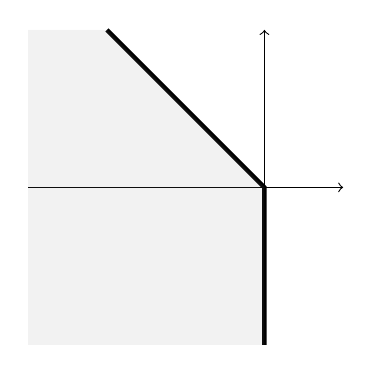
\begin{tikzpicture}
                \draw [->] (-3,0) -- (1,0);
                \draw [->] (0,-2) -- (0,2);
                \draw [ultra thick] (-2,2) --(0,0)--(0,-2);
                \path [fill=gray, fill opacity=.1] (-3,2)--(-2,2) --(0,0)--(0,-2)--(-3,-2)--(-3,2);
            \end{tikzpicture}
            \caption{convex cone}
        \end{subfigure}%
        \begin{subfigure}{.5\textwidth}
            \centering
            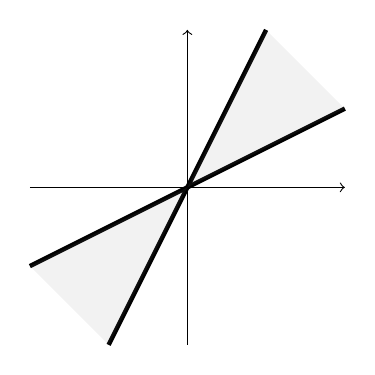
\begin{tikzpicture}
                \draw [->] (-2,0) -- (2,0);
                \draw [->] (0,-2) -- (0,2);
                \draw [ultra thick] (1,2)--(-1,-2);
                \draw [ultra thick] (2,1)--(-2,-1);
                \path [fill=gray,fill opacity=.1] (1,2)--(0,0)--(2,1)--(1,2);
                \path [fill=gray,fill opacity=.1] (-1,-2)--(0,0)--(-2,-1)--(-1,-2);
            \end{tikzpicture}
            \caption{violation of convex cone}
        \end{subfigure}
    \end{figure} 

    \item[13.] Additivity: $y,y' \in Y \implies y + y' \in Y$
    \begin{figure}[H]
        \centering
        \begin{subfigure}{.5\textwidth}
            \centering
            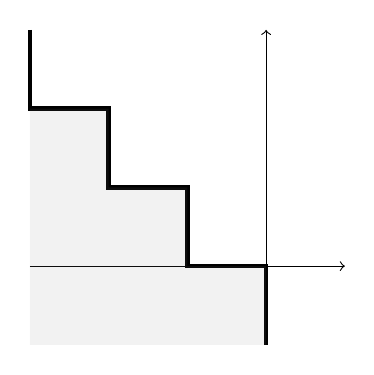
\begin{tikzpicture}
                \draw [->] (-3,0) -- (1,0);
                \draw [->] (0,-1) -- (0,3);
                \draw [ultra thick] (-3,3)--(-3,2)--(-2,2)--(-2,1)--(-1,1)--(-1,0)--(0,0)--(0,-1);
                \path [fill=gray, fill opacity=.1] (-3,3)--(-3,2)--(-2,2)--(-2,1)--(-1,1)--(-1,0)--(0,0)--(0,-1)--(-3,-1)--(-3,3);
            \end{tikzpicture}
            \caption{additivity}
        \end{subfigure}%
        \begin{subfigure}{.5\textwidth}
            \centering
            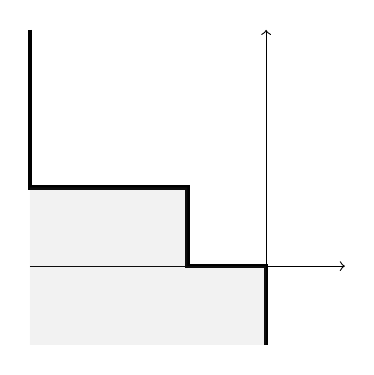
\begin{tikzpicture}
                \draw [->] (-3,0) -- (1,0);
                \draw [->] (0,-1) -- (0,3);
                \draw [ultra thick] (-3,3)--(-3,1)--(-1,1)--(-1,0)--(0,0)--(0,-1);
                \path [fill=gray,fill opacity=.1] (-3,3)--(-3,1)--(-1,1)--(-1,0)--(0,0)--(0,-1)--(-3,-1)--(-3,3);
            \end{tikzpicture}
            \caption{violation of additivity}
        \end{subfigure}
    \end{figure} 
\end{enumerate}

\end{document}
